\documentclass[tikz,border=10pt]{standalone}
% Semicircle MN with centre O, radius OP, point A on OP, point B on arc
\usepackage{amsmath}
\begin{document}
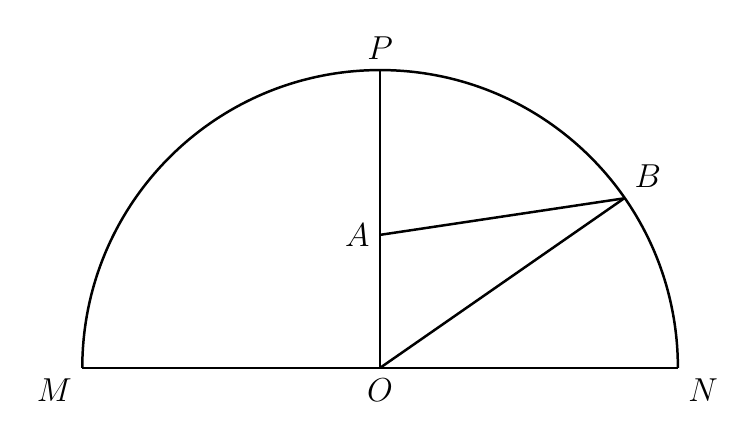
\begin{tikzpicture}[line join=round, line width=0.9pt, font=\fontsize{12.5}{15}\selectfont]
  % Coordinates: O at origin, scale 0.016064 cm per px, radius R = 3.782 cm
  \coordinate (O) at (0,0);
  \coordinate (M) at (-3.782,0);
  \coordinate (N) at (3.782,0);
  \coordinate (P) at (0,3.782);
  \coordinate (A) at (0,1.689);
  \coordinate (B) at (3.100,2.153);

  % Baseline MN (solid)
  \draw (M) -- (N);

  % Upper semicircle from N through P to M (not a full circle)
  \draw (N) arc[start angle=0, end angle=180, radius=3.782];

  % Radius OP (solid), segments OB and AB (solid)
  \draw (O) -- (P);
  \draw (O) -- (B);
  \draw (A) -- (B);

  % Labels outside strokes
  \node[below left] at (M) {$M$};
  \node[below] at (O) {$O$};
  \node[below right] at (N) {$N$};
  \node[above] at (P) {$P$};
  \node[left] at (A) {$A$};
  \node[above right] at (B) {$B$};
\end{tikzpicture}
\end{document}